\documentclass{article}
\usepackage[margin=1in]{geometry}
\usepackage{array}
\usepackage{graphicx}
\usepackage{natbib}
\usepackage{amsmath, amssymb}

\author{Carl Ehrett}
\title{Computer model calibration as a method of design}

\begin{document}

\maketitle

\section{Introduction} \label{introduction}
% Discussion of computer experiments and computer model calibration. Lit review. Overview of project goals.

\subsection{Computer experiments} \label{computer_experiments}

Suppose that one wishes to improve one's understanding of, say, the movement of people in a crowd escaping from a building in a crisis situation. This is an example of an area in which field data are extremely difficult to acquire. Merely assembling a crowd of research subjects in one place is costly and difficult. Asking them to flee a building may result in behaviors which are unlike those in real crisis situations -- but which may nonetheless present unacceptable physical risk to the subjects. Inducing them to flee through the generation of a (real or apparent) crisis is similarly infeasible. Observational data are likewise scarce here, since panic-inducing crises are by their nature difficult to predict and chaotic in ways that hinder the reliable collection of data.

In the face of these difficulties, computer models offer an alternative to the choice between attempting field data collection and giving up on the hope of progress. Using existing theory concerning human psychology and movement, it is possible to construct a computer model simulating the behavior of people evacuating from a large building. For example, the SIMULEX model described by \cite{Thompson1995} allows one to observe simulated evacuation behaviors in any specified building layout, using any desired physical distribution of individuals, whose individual relevant characteristics (walking speed, initial bodily orientation, etc) may be controlled by the researcher. Thus, computer models provide a means to collect data which might otherwise be largely inaccessible. 

The study of computer models from a statistical perspective calls for specialized tools and techniques. Gaussian processes (GPs) are a popular tool for modeling the output of computer code. There are three reasons for this popularity: (1) The use of a GP does not require detailed foreknowledge of the approximate parametric form of the computer model. Researchers often lack such foreknowledge in the case of complex computer models. (2) GPs easily interpolate the observed data. This is an advantage when the observations come from deterministic computer code that is free of observation error. (3) The variance of a GP provides a natural form of uncertainty quantification. 
A Bayesian approach to the study of computer models is undertaken by \cite{Currin1991}; the authors approach GPs as prior distributions on the unknown form of the computer model. A frequentist applications of GPs to computer models is provided by \cite{Sacks1989}, who use GPs not only for estimating uncertainty but also as the basis for their approach to experimental design in the area of deterministic computer models.  \cite{Santner2003a} offer a comprehensive discussion of to the use of GPs for prediction, design, and sensitivity analysis with respect to computer experiments from both frequentist and Bayesian perspectives. It is against the background of these works that the past two decades of research into computer model calibration takes place.

\subsection{Computer model calibration} \label{computer_model_calibration}

Suppose that we wish to use the SIMULEX model to compare two different proposed building codes to be enforced in, say, St.\ Louis, Missouri. We may use average walking speed and average interpersonal distance as input parameters for this model, both to settle the initial physical distribution of people throughout the building and to influence their behavior during evacuation. It is well-established that average walking speed \citep{Bornstein1976} and interpersonal distance \citep{Sorokowska2017} vary across locales. These values may be unknown for the case of St.\ Louis. Thus we may wish to find the true values for average walking speed and interpersonal distance in St.\ Louis; we may wish, in other words, to \textit{calibrate} these parameters in the model.

Broadly, in model calibration, we may consider a model to be of the form $\eta(x,\theta)$, where $(x,\theta)$ comprise all inputs to the model. Control inputs --- inputs under the control of the researcher (in the evacuation example, this would include the building layout) comprise $x$, whereas $\theta$ is the set of calibration inputs --- parameters the values of which are not under researcher control, but rather are unknown values which must be estimated for successful simulation. Thus where $f$ describes the true system, we consider the model to be 
\begin{equation} \label{eq:1}
f(x,\theta)=f(x)=\eta(x,\theta) + \delta(x)
\end{equation} 
where $\delta$ describes the model discrepancy -- i.e., the bias of the model as an estimate of the real system. Notice that we may write $f(x)=f(x,\theta)$ since $\theta$ does not vary in reality. To undertake model calibration, we must have access to at least some observations of the real system; it is to these real observations that we calibrate the computer model.

Much interest in the past two decades has centered on Bayesian methods for model calibration. The appeal of a Bayesian approach to model calibration lies in the fact that the calibration parameters are a source of uncertainty for the model. This uncertainty should be quantified so that its effect on the model can be made explicit. We can thus use Bayesian methods to arrive at a posterior distribution on the calibration parameters which balances our prior knowledge about the calibration parameters with what can be learned from the available data, and which also allows for accurate uncertainty quantification on the model outputs. 

The work of \cite{Kennedy2001} has been influential in this area. Kennedy and O'Hagan offer a Bayesian approach to computer model calibration that allows for the uncertainty of the calibration parameters in the predictions of the resulting calibrated model. This area is furthered by \cite{Higdon2004}, who develop an approach that undertakes model calibration with quantification of the related uncertainty, as well as explicitly incorporating uncertainty regarding the computer model output, the bias of the computer model, and uncertainty due to observation variance (of field data). That approach is further refined and exemplified by \cite{Williams2006}.
\cite{Loeppky2006} offer an MLE-based alternative to the Bayesian approach promulgated by Kennedy and O'Hagan, intending thereby to improve the identifiability of the calibration parameters in the face of model discrepancy. 
\cite{Bayarri2007} extends the approach of Kennedy and O'Hagan, providing a framework that is intended to allow for simultaneous validation and calibration of a computer model (using the same training data). Though they  work within the Bayesian framework set by Kennedy and O'Hagan, they mitigate the integrity of the Bayesian analysis through what they call ``modularization''. Modularization refers to separating sources of information, so that the model has distinct components or ``modules'', rather than allowing all information to combine into a single analysis under the umbrella of Bayes' theorem. \cite{Liu2009} focus directly on the use of modularization, exploring its advantages and disadvantages; amongst other potential motivations, they show that modularization can improve the identifiability of calibration parameters. 
\cite{Bayarri} furthers the project of \cite{Bayarri2007} by applying the latter's methodology to functional data. To do so, the methodology for dealing with scalar data is hierarchically applied to the coefficients of a wavelet representation of the functional data. Similarly, \cite{Paulo2012} focuses on applying the lessons of \cite{Bayarri2007} to computer models with multivariate output.

Above, I have described model calibration as a matter of estimating the true values of unknown parameters. Indeed, that is the sort of model calibration that will form the focus on the present work. However, in a broad sense of the term, model calibration takes a second form as well. For convenience, we may distinguish this second form by referring to it as \emph{tuning}, rather than as calibration. In model tuning, a computer model includes inputs which must be calibrated, but which have no particular interpretation; i.e., tuning parameters do not represent the truth regarding some value of the system being modeled. The work of \cite{Brynjarsdottir2014} emphasizes the distinction between calibration and tuning. They show that whereas a well-modeled discrepancy function ($\delta(\cdot)$ in Equation \ref{eq:1}) may not be necessary for tuning, since the tuning process can accomplish much of the work of a discrepancy function, an accurate discrepancy function is crucial for calibration, for the same reason. Letting the calibration process take on the duties of the discrepancy function reduces the identifiability of the calibration parameters.

Another extension of the framework of \cite{Kennedy2001} and \cite{Bayarri2007} is the \emph{state-aware} calibration of \cite{Brown2016}. When one knows or suspects that the appropriate value of a calibration parameter $\theta$ is dependent upon the other inputs $x$, state-aware calibration allows for the calibration procedure to estimate $\theta$ as $\theta(x)$. This may obviate the need for a discrepancy function, either because the true value of the calibration parameter does indeed vary with the other inputs, or (in a tuning problem) because varying the tuning parameter can accomplish the work of a discrepancy function in aligning the computer model response with reality.

\subsubsection{Gaussian processes} \label{gaussian_processes}

In principle, model calibration\footnote{In this work, ``calibration'' will usually be used broadly to include model tuning; where it is used in such a way as to exclude tuning, this will be made clear in context.}
need not rely on a GP emulator, or any other sort of emulator; one could (e.g.) complete a full Bayesian analysis via an MCMC chain that involves running the relevant computer model at each iteration of the chain. However, computer models are frequently too computationally expensive to allow for such profligacy. Instead, a computationally tractable emulator can be constructed using a sample of observations from the computer model. As described in Section \ref{computer_experiments}, GPs are popular prior distributions on computer model output, because (1) their use does not require detailed foreknowledge of the model function's parametric form, (2) GPs easily interpolate the (deterministic) computer model output, and (3) GPs facilitate uncertainty quantification through the variance of the posterior GP. In this section, I provide brief background on Gaussian processes and their use in regression broadly and in computer model calibration specifically.

%\paragraph{Background}

Gaussian processes can be thought of as generalizations of multivariate normal random variables. Whereas a multivariate normal random variable is a random vector of finite length, a Gaussian process can be thought of as a random function. The value of the function at any finite selection of points is itself a multivariate normal random variable. Just as a multivariate random variable is characterized by its mean vector and covariance matrix, a Gaussian process is fully characterized by its mean function $\mu:D\to \mathbb R$ and covariance function $C:D\times D\to \mathbb R$, where $D$ is the domain of the process. Thus for any points $x,y$ in the domain of the Gaussian process, $\mu(x)$ gives the mean of the Gaussian process at $x$, and $C(x,y)$ gives the covariance between the values of the Gaussian process at points $x$ and $y$. As a special case, then, $C(x,x)$ gives the marginal variance of the GP at $x$. 

%\paragraph{Gaussian process regression}

\cite{OHagan1978} suggested the use of GPs as priors for modeling unknown functions. Given observations $\mathbf f$ from the function $f$ being modeled, an updated mean and covariance function $\mu^*(x)=\mu(x)|\mathbf f$ and $C^*(x,y) = C(x,y)|\mathbf f$ describe a new GP that has been ``trained'' on the observations $\mathbf f$. O'Hagan did not focus in that work on applications to computer models. The use of GPs to produce a computationally efficient predictor $\hat \eta (x)$ of expensive computer code $\eta(x)$ given observations of code output at $\mathbf x=\{x_i\}_{i=1}^n$ is promulgated by \cite{Sacks1989} and explored at length by \cite{Santner2003a}. Since computer code is typically deterministic, these applications differ from O'Hagan's focus in that the updated GP is induced to interpolate the observations $\boldsymbol \eta = (\eta(x_1),\cdots,\eta(x_n))^T$. The updated mean allows for prediction of the computer model at points not observed, with uncertainty quantified by the updated covariance function.

Suppose, for example, that we begin with a prior GP with constant mean function $\mu(x)=0\ \forall x$. Notice that we may use our covariance function $C$ to define an $n\times n$ matrix $\mathbf C_{\mathbf x,\mathbf x}$ such that the $i,j$ entry of $\mathbf C_{\mathbf x,\mathbf x}$ is equal to $C(x_i,x_j)$. We may wish to train our GP on these $n$ observations, and then examine the resulting posterior GP at the points $\mathbf x'=\{x_i' \}_{i=1}^m$. Recall that the GP at the points $\mathbf x'$ is a multivariate normal random variable of length $m$, which is fully characterized by its mean vector $\mu^*_{\mathbf x'}$ and covariance matrix $\mathbf C^*_{\mathbf x',\mathbf x'}$. We can find these as:
\begin{equation}\label{eq:post_gp}\begin{split}
\mu^*_{\mathbf x'}&=\mathbf C_{\mathbf x',\mathbf x}\cdot \mathbf C_{\mathbf x,\mathbf x} ^{-1}\cdot \boldsymbol \eta
\\
\mathbf C^*_{\mathbf x'}&=\mathbf C_{\mathbf x',\mathbf x'}-\mathbf C_{\mathbf x',\mathbf x}\cdot \mathbf C_{\mathbf x,\mathbf x}^{-1}\cdot \mathbf C_{\mathbf x,\mathbf x'}
\end{split}\end{equation}
A visualization of this example can be found in Figure \ref{fig:gp_example}. Here, $n=5$, and $x'=(-5,-4.75,⋯,4.75,5)$. 

\begin{figure}[h]
\centering
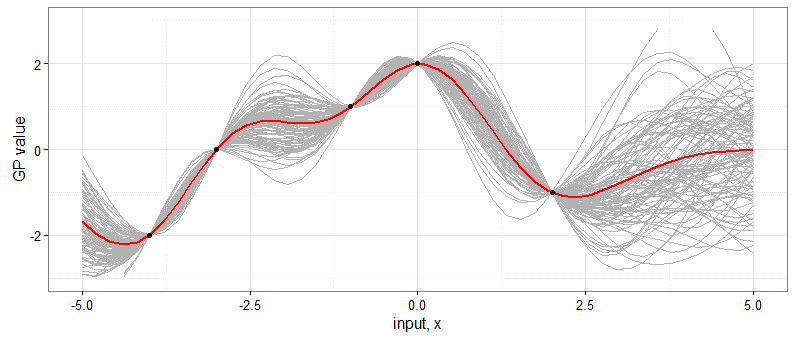
\includegraphics[width=.75\linewidth]{gp_example}
\caption{Example of a Gaussian process trained to interpolate five data points (black dots). The posterior mean function is shown in red; the gray lines are 50 draws from the posterior GP.}
\label{fig:gp_example}
\end{figure}

Though the approach of \cite{OHagan1978} was Bayesian, it did not provide for Bayesian means of selecting a covariance function $C$. \cite{Neal} extends the work of O'Hagan in this direction. \cite{Savitsky2011} describes a method for variable selection in GP regression via spike-and-slab mixture priors on the parameters of the covariance function. \cite{Shang2013} provide an umbrella generalization of existing methods of GP regression under a framework of what they call generalized GP models. All of these works treat GP regression generally, and do not focus specifically on the use of GPs to build emulators for computer model.

By contrast, much recent attention following the work of \cite{Santner2003a} and \cite{Sacks1989} has focused specifically on the use of GPs for computer model emulation. 
\cite{Kennedy2001} themselves develop an influential framework for Bayesian analysis using GPs specifically for computer model calibration. \cite{Kennedy2006} showcase this use of GP emulators for uncertainty and sensitivity analyses. \cite{Bastos2009} describes both numerical and graphical diagnostic techniques for assessing when a GP emulator of a computer model is successful, as well as discussion of likely causes of poor diagnostic results. While most work in the area of GP emulation uses stationary covariance functions (in which $C(x,y)=C(|x-y|)$ depends only on the distance between $x$ and $y$, and not on their location in the input domain) and quantitative inputs, efforts have been made to branch away from these core uses. \cite{Gramacy2008} use treed partitioning to deal with a nonstationary computer model. \cite{Qian2008} explore methods for using GP emulators that include both quantitative and qualitative inputs.

%\paragraph{Gaussian processes in computer model calibration}

Aside from \cite{Kennedy2001}, recent applications of GP emulation specifically to problems of calibration have focused largely on the works of \cite{Williams2006} and \cite{Bayarri2007}. It will be helpful here to provide an illustrative summary of the approach taken by \cite{Williams2006}, both to exemplify the use of GPs for computer model calibration and because the approach utilized in the present work closely follows theirs.

Consider that we have inputs $x\in \mathbb R^p$ and $t\in\mathbb R^q$ scaled to the unit hypercube, and observations 
\begin{equation}\label{eq:2}
y(x_i) = f(x_i) + \epsilon(x_i),\quad i=1,\cdots,n,
\end{equation}
where $f(\cdot)$ is the true system and $\epsilon(x_i)$ is known measurement error. Then by Equation \ref{eq:1} we have
\begin{equation}\label{eq:2}
y(x_i) = \eta(x_i,\theta) + \delta(x_i) + \epsilon(x_i),\quad i=1,\cdots,n
\end{equation}
where $\eta(\cdot,\cdot)$ is the computer model, $\theta$ is the best\footnote{In the case of calibration, the ``best'' setting will be the true setting of that parameter; in a case of tuning rather than calibration, the ``best'' setting would instead be the optimal setting for minimizing model bias.}
setting of the vector of calibration parameters, and $\delta(\cdot)$ is the discrepancy function describing the bias of $\eta(\cdot,\cdot)$ as an estimate of $f(\cdot)$.

\citeauthor*{Williams2006} define the GP prior for modeling $\eta(\cdot,\cdot)$ as follows. Let the mean function $\mu(x,t)=c$, $c$ a constant. Set the covariance function to have the (stationary) form 
\begin{equation}\label{eq:Hig_cov}
C((x,t),(x',t')) = \frac 1\lambda_\eta \prod_{k=1}^{p}
\exp \left(-\beta^\eta_k|x_k-x_k'|^{\alpha_\eta}\right) \times
\prod_{k=p+1}^{p+q}
\exp \left(-\beta^\eta_{k}|t_k-t_k'|^{\alpha_\eta}\right)
\end{equation}
where $\lambda_eta$ is the marginal precision of the GP; each $\beta_k$ describes the strength of the GP's dependence on one of the elements of the input vectors $x,t$; and $\alpha_\eta$ describes the smoothness of the GP. 

The authors place the following priors on the hyperparameter:
\begin{align}
\pi (c) &\sim N(0,v)\\
\pi(\lambda_\eta) &\sim \mathrm{Gamma}(5,5),\quad\lambda_\eta>0\\
\pi\left(\rho_k^\eta\right) &\sim \mathrm{Beta}(1,0.1),\quad k=1,\cdots,p+q
\end{align}
where $\rho_k^\eta=\exp(-\beta_k^\eta)/4)$ $\forall k$. The parameters of the Gamma and Beta distributions are chosen to encourage $\lambda_\eta$ to be close to one, and $\beta_k$ to be low for all $k$ (encouraging strong dependence; i.e., we antecedently expect each of our inputs to be influential). Furthermore, the authors let $v\to0$, i.e., the GP is assumed to have constant mean $c=0$.

The authors similarly model the discrepancy term as a GP, also with mean zero, and covariance function
\begin{equation}
C_\delta(x,x') = \frac 1{\lambda_\delta} \prod_{k=1}^p
\exp\left( -\beta_k^\delta |x_k-x_k'|^{\alpha_\delta} \right),
\end{equation}
with priors
\begin{align}
\pi(\lambda_\delta) &\sim \mathrm{Gamma}(a_\delta,b_\delta)\\
\pi(\rho^\delta_k) &\sim \mathrm{Beta}(1,0.3).
\end{align}
where $\rho_k^\delta=\exp(-\beta_k^\delta/4)$ $\forall k$.

Then where $\boldsymbol \eta = (\eta(x_1,t_1),\cdots,\eta(x_n,t_n))^T$ are the simulation observations, $\mathbf y = (y(x_{n+1}),\cdots,y(x_{n+m}))^T= (y(x_{n+1},\theta),\cdots,y(x_{n+m},\theta))^T$ are the field observations, $\mathcal D = (\mathbf y^T \boldsymbol \eta^T)^T$, $\boldsymbol \beta^\eta = (\beta^\eta_1,\cdots,\beta_{p+q}^\eta)^T$, and $\boldsymbol \beta^\delta = (\beta^\delta_1,\cdots,\beta_{p+q}^\delta)^T$, we have the distribution of $\mathcal D$ as
\begin{equation}
\mathcal D | \theta,c,\lambda_\eta, \beta^\eta,\lambda_\delta,\beta^\delta,\mathbf C_y \sim N(c \cdot \mathbf 1_{n+m}, \mathbf C_{\mathcal D})
\end{equation}
where $\mathbf C_y$ an $m\times m$ matrix in which the $i,j$ entry is the (known) observation variance $C_{obs}(x_i,x_j)$ for $n<i,j\leq n+m$, and $\mathbf C_{\mathcal D}$ is a matrix with its $i,j$ entry equal to
\begin{equation}
C((x_i,t_i),(x_j,t_j)) + I(i,j>n)\cdot(C_{obs}(x_i,x_j) + C_\delta(x_i,x_j))
\end{equation}
Thus, the joint posterior density given by the model is
\begin{equation} \label{eq:full_dist}
\pi(\theta,c,\lambda_\eta,\rho^\eta,\lambda_\delta,\rho^\delta|\mathcal D)
\propto \pi(\mathcal D | \theta,c,\lambda_\eta, \beta^\eta,\lambda_\delta,\beta^\delta,\mathbf C_y) \times \pi(c) \times \pi(\lambda_\eta) \times 
\pi(\rho^\eta) \times \pi(\lambda_\delta) \times \pi(\rho^\delta)
\end{equation}
Note that where a discrepancy function is not included in the model and the mean $c$ is treated as a constant, (\ref{eq:full_dist}) simplifies greatly; where furthermore $\lambda_\eta$ and $\rho^\eta$ are estimated via maximum likelihood (as in  \cite{Kennedy2001}),  (\ref{eq:full_dist}) simplifies down merely to 
$\pi(\mathcal D | \theta,c,\lambda_\eta, \beta^\eta,\lambda_\delta,\beta^\delta,\mathbf C_y)$. Markov chain Monte Carlo methods are useful for evaluating (\ref{eq:full_dist}); the next section takes up this topic.

\subsubsection{Markov chain Monte Carlo methods}

%\paragraph{Background}

The central idea of Markov chain Monte Carlo (MCMC) integration is to construct a Markov chain which has as its equilibrium distribution the target distribution one wishes to explore. The Markov chain is observed, and beyond an initial ``burn-in'' period during which the chain is allowed to approach its equilibrium distribution, samples are considered to be drawn approximately from the target distribution.

For example, consider a model with full distribution given by (\ref{eq:full_dist}), but where discrepancy is not included and $\lambda_\eta,\rho^\eta$ are found via maximum likelihood estimation. Then the full distribution is given by $\pi(\theta,c,\lambda_\eta,\rho^\eta,\lambda_\delta,\rho^\delta|\mathcal D)
\propto \pi(\mathcal D | \theta,c,\lambda_\eta, \beta^\eta,\lambda_\delta,\beta^\delta,\mathbf C_y) \times \pi(c)$. A simple means of exploring this distribution via MCMC would begin with an initial guess $\theta^{(1)},c^{(1)}$. At the $i^{\text{th} }$ step for $i=2,\cdots$, using a proposal distribution $\pi_{prop}(\cdot,\cdot|{\theta^{(i-1)},c^{(i-1)}})$ from which we may easily sample directly, we draw a new ``proposed'' sample $\theta^*,c^*$. We then with probability $\alpha$ accept this new proposed sample, setting $(\theta^{(i)},c^{(i)}) = (\theta^*,c^*)$; otherwise we reject the proposed sample and let $(\theta^{(i)},c^{(i)}) = (\theta^{(i-1)},c^{(i-1)})$. In doing so, we have 
\begin{equation}\label{eq:mh-acceptance}
\alpha = \frac{\pi(\theta^*,c^* | \mathcal D)}{ \pi(\theta^{(i-1)},c^{(i-1)}|\mathcal D) } = 
\frac{ \pi(\mathcal D | \theta^*,c^*,\lambda_\eta, \beta^\eta,\lambda_\delta,\beta^\delta,\mathbf C_y) \times \pi(c^*)}{\pi(\mathcal D | \theta^{(i-1)},c^{(i-1)},\lambda_\eta, \beta^\eta,\lambda_\delta,\beta^\delta,\mathbf C_y) \times \pi(c^{(i-1)})}
\end{equation}
Note that in order to proceed in this way, it is necessary that $\pi_{prop}$ be a symmetric distribution. The version of MCMC described in this example is known as the Metropolis-Hastings algorithm; it was initially described by \cite{Metropolis1953} and generalized by \cite{Hastings1970}. A thorough exposition of the technique, its theoretical foundation, and its relation to other  varieties of MCMC is provided by \cite{Chib1995}.

% Gibbs
A related variant of MCMC -- in fact, a special case of Metropolis-Hastings, as shown by \cite{Gelman1992} -- is Gibbs sampling, initially described by \cite{Geman1984}. In using Gibbs sampling, one finds the conditional distribution of each of the parameters one wishes to sample, using the most recent samples of all other parameters. For example, we can convert the above Metropolis-Hastings illustration to a simple case of Gibbs sampling as follows.
Begin as before, with initial guesses $\theta^{(1)}$ and $c^{(1)}$. Thereafter, sample $\theta$ and $c$ not together, but rather in alternating draws. That is, at the $i^{\text{th} }$ step for $i=2,\cdots$, draw $\theta^{(i)}$ conditional on $c=c^{(i-1)}$, then draw $c^{(i)}$ conditional on $\theta=\theta^{(i)}$. Thus, for example, when drawing $c^{(i)}$, its conditional distribution would be proportional to $\pi(\mathcal D | \theta^{(i)},c^{*},\lambda_\eta, \beta^\eta,\lambda_\delta,\beta^\delta,\mathbf C_y) \times \pi(c^{*})$. 
If the conditional distribution is something from which we may easily draw directly, then we can draw $c^{(i)}$ that way; otherwise, we can use a so-called Metropolis-within-Gibbs scheme, and draw $c^{(i)}$ similarly to what was described above for the Metropolis-Hastings algorithm: draw a proposed $c^*$ from a proposal distribution, find the appropriate ratio $\alpha_c$, and accept or reject $c^*$ accordingly. In the application considered in the present work, Metropolis-within-Gibbs will be used.

%\paragraph{Elimination of boundary constraints}

Recall that a symmetric proposal distribution is required in order for the Metropolis-Hastings algorithm to proceed as described in the above illustration of that technique. However, the algorithm can accommodate an asymmetric proposal distribution with only slight complication. A frequent reason for using an asymmetric proposal distribution is the existence of boundary constraints on the parameter being sampled. Thus, for example, in the application considered in the present work, one of the calibration parameters is the thickness (in mm) of the material forming a wind turbine blade. Expert opinion was used to set the support of this parameter to be the range [10mm, 25mm]. Good mixing in the MCMC chain is promoted by choosing a proposal density such that the distribution $\pi_{prop}(\cdot|\tau)$ has mean $\tau$. With boundary constraints, this requires an asymmetric distribution. When $\pi_{prop}(\cdot|\tau)$ is asymmetric, this changes the above illustration only by way of requiring us to calculate the acceptance probability $\alpha$ as follows:
\begin{equation}\label{eq:mh-correction}
\alpha = \frac{\pi(\theta^*,c^* | \mathcal D)}{ \pi(\theta^{(i-1)},c^{(i-1)}|\mathcal D) } \times 
\frac{
\pi_{prop}(\theta^{(i-1)},c^{(i-1)}|\theta^*,c^*)
}{
\pi_{prop}(\theta^*,c^*|\theta^{(i-1)},c^{(i-1)}).
}
\end{equation}

%\subsubsection{Normalization of inputs and standardization of outputs}
%Blah

\subsubsection{Computational difficulties}
% And solutions
Note that the joint posterior density given in (\ref{eq:full_dist}) above includes $\mathbf C_{\mathcal D}$, which, depending on how many field and simulation observations one has, may be of fearsomely high dimension. This can lead to computational difficulties in calculating $\alpha$ in the course of the MCMC routine. Difficulties arise in two ways. Firstly, the likelihood given in (\ref{eq:full_dist}) evaluated at a given point can be so small as to be vulnerable to significant round-off error. Secondly, the poor conditioning of $\mathbf C_{x,x}$ in (\ref{eq:post_gp}) can make it difficult to invert. The latter problem can be alleviated by adding a small nugget to $\mathbf C_{x,x}$; i.e., (abusing notation somewhat) we can set $\mathbf C_{x,x}= \mathbf C_{x,x} + \xi \cdot \mathbf I_{\mathrm{dim}(\mathbf x)}$

\paragraph{Likelihoods}
Blah

\paragraph{Ill-conditioned covariance matrices}

\section{Calibration for design}



\section{Application}

\subsection{Project background}

\subsection{Emulation of finite element simulator}
Blah

\subsubsection{Wind turbine blade simulator}
% Here the finite element model will be described
Blah

\subsubsection{Mathematical basis for the emulator}
% Includes formulae for trained mean and covariance functions
Blah

\subsubsection{Experimental design}
% How we selected the design points at which to observe the simulator
Blah

\subsubsection{Covariance parameters}
% How they were selected
Blah

\paragraph{Finding covariance parameters via MCMC}
% Why we didn't do it (computational difficulties
Blah

\paragraph{Grid optimization}
% Advantages and disadvantages; full grid and integration of lambda
Blah

\paragraph{Gradient method}
% Explanation and advantages
Blah

\begin{figure}
\centering
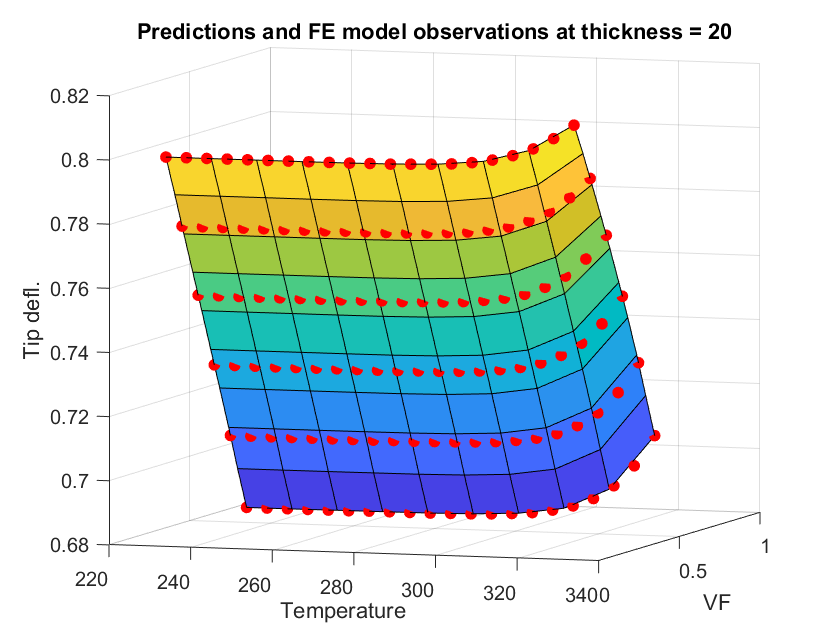
\includegraphics[width=.65\linewidth]{emulator_surface}
\caption{A slice of the GP emulator (restricted to the output for tip deflection) at thickness =20mm. Red dots are observations from the simulator.}
\label{fig:emulator_surface}
\end{figure}

\section{MCMC using the emulator}
Blah

\subsection{MCMC methods}
% Background on MCMC
Blah

\subsection{The model}
% Choice of priors and resulting likelihood
Blah

\subsubsection{Desired observation variance}
% 4 versions: heterosked constant, homosked constant, heterosked prior, homosked prior
\begin{table}[h]
\centering
\begin{tabular}{| c | c  |  c  | c |  c  |}
\hline
 \vspace{-3mm}
& & & & \\
& \parbox{24mm}{\centering Heteroskedastic, constant}& \parbox{24mm}{\centering Homoskedastic, constant}& \parbox{24mm}{\centering Heteroskedastic, prior} & \parbox{24mm}{\centering Homoskedastic, prior}\\
 \vspace{-3.5mm}
& & & & \\
\hline
Deflection & 0.749 & 0.729 & 0.659 & 0.709\\
Rotation & 0.0904 & 0.0865 & 0.0773 & 0.0843\\
Cost & 276.16 & 236.11 & 350.80 & 233.95 \\
\hline
\end{tabular}
\caption{Comparison of model outputs, where the desired data outputs are assumed to be either homoskedastic or heteroskedastic, with either a specified constant variance or a $1/\sigma^2$ prior.}
\label{table:obs_var_comp}
\end{table}

\begin{figure}
\centering
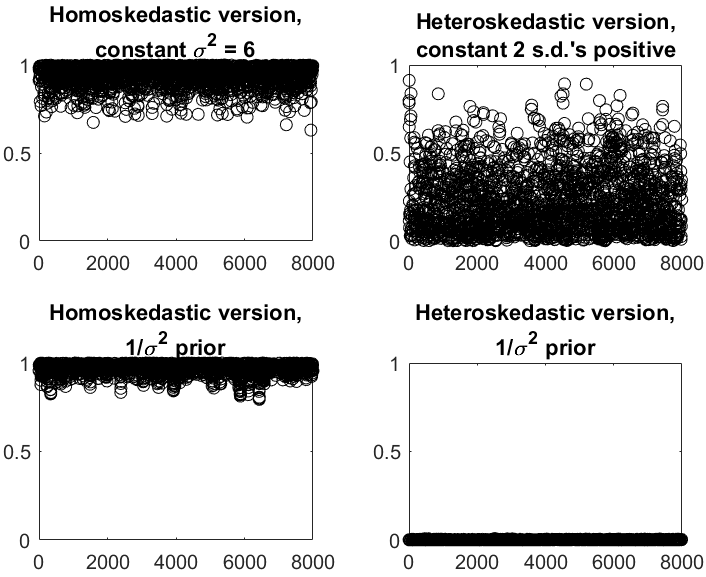
\includegraphics[width=.65\linewidth]{comp_obs_var}
\caption{MCMC results at various observation variance settings.}
\label{fig:comp_obs_var}
\end{figure}

\subsubsection{Full model and likelihood}
Blah

\subsubsection{Convergence difficulties}
% And the idea to eliminate boundary constraints
Blah

\subsubsection{Implementation of the Metropolis-Hastings algorithm}
Blah

\begin{figure}
\centering
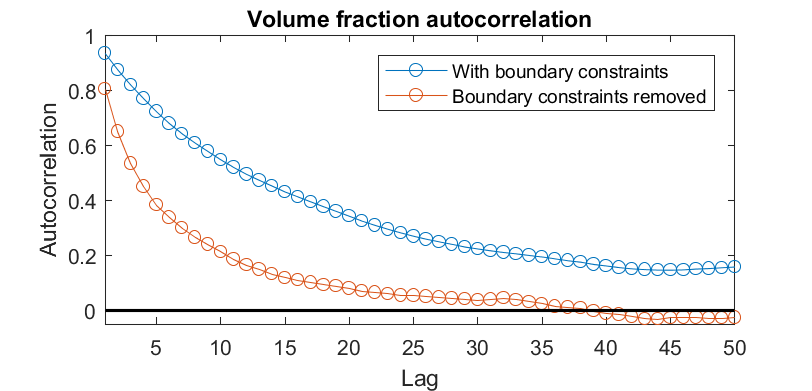
\includegraphics[width=.9\linewidth]{ACF_bnd_cnds_fig}
\caption{Auto-correlation for draws both with and without the elimination of boundary conditions.}
\end{figure}

\subsection{Which data to desire?}
Blah

\subsubsection{Motivations behind the choice of desired data}
Blah

\subsubsection{Differing results}
% for different desired data values
\begin{table}[h]
\centering
\begin{tabular}{| c | c  | c  |  c | c  | c | c | c |}
\hline
Desired data $d$ & $\sigma^2_{defl}$ & $\sigma^2_{rot}$ & $\sigma^2_{cost}$ & $\mu_{v|d}$ &
                            $\mu_{h|d}$ & $\sigma^2_{v|d}$ & $\sigma^2_{h|d}$\\
\hline
$(0, 0, 0)$ & 375.45 & 277.69 & 2.62 & 0.215 & $4.01 \cdot 10^{-2}$&
	$4.41\cdot 10^{-2}$ & $1.92 \cdot 10^{-3}$\\
$(0.65, 0.077, 96)$ & 16.74 & 15.25 & $4.62 \cdot 10^{-7}$ &
	$1.09 \cdot 10^{-3}$ & $3.36 \cdot10^{-4}$ &
	$1.02 \cdot 10^{-5}$ & $9.97 \cdot 10^{-6}$\\
\hline
\end{tabular}
\caption{Comparison of results for two different (low) values of $d$. Values listed are, respectively, the posterior means for the observation variance of each model output, posterior means for volume fraction ($v$) and thickness ($h$), and posterior variance of volume fraction and thickness.}
\label{table:d_comp}
\end{table}

\begin{figure}
\centering
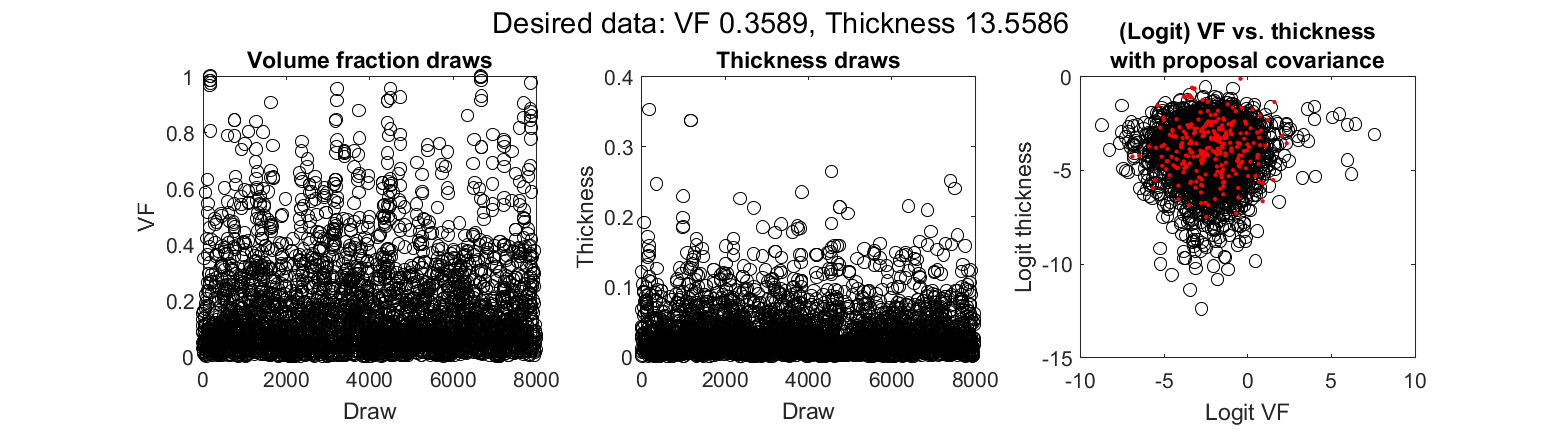
\includegraphics[width=.9\linewidth]{FIG1}
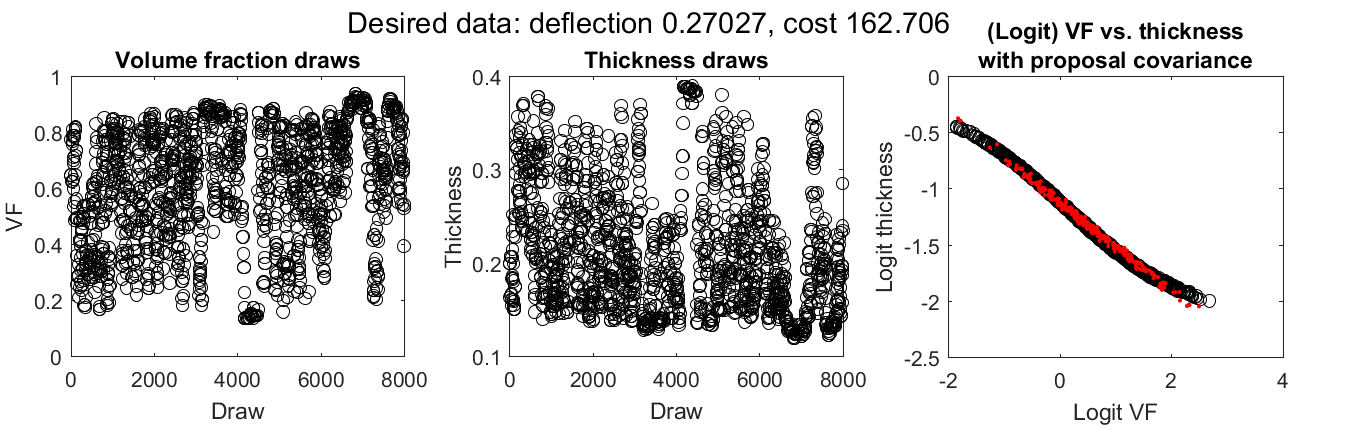
\includegraphics[width=.9\linewidth]{FIG2}
\caption{MCMC results for low deflection and cost (top row) and low deflection with easily achievable cost (bottom row).}
% NOTE: THESE PLOT TITLES ARE WRONG! GOTTA DO THE PLOTS OVER! LOL!
\label{fig:des_data}
\end{figure}

\subsection{Exponentially distributed desired data}
Blah

\subsubsection{Motivation}
Blah

\subsubsection{Implementation and results}
Blah


\subsection{Identifiability issues}
% Issues arising from the non-identifiability of VF, thickness when cost is relaxed
Blah

\section{Future work}
Blah

\subsection{Alternative means of handling cost}
Blah

\subsubsection{Removing cost from the model}
Blah

\subsubsection{Alternative priors for controlling cost}
Blah

\subsection{Building a desired data response surface}
Blah

\subsection{Implementing Hamiltonian Monte Carlo}
Blah

\subsubsection{Hamiltonian Monte Carlo}
% Background
Blah

\subsubsection{Benefits}
Blah

\subsection{Model discrepancy}
% Include (or investigate the inclusion of) a model discrepancy function
Blah

\section{Conclusion}
% Discussion of the role of computer model validation as a potential methodology for design
Blah












\bibliographystyle{authordate1}
% This style file is a version of the plain.bst style file which I edited myself to add abstract and annotation fields.

\bibliography{lit_review}

\end{document}